

\chapter{Nuclear}

Hola

\section{Estadística}

\section{Interacción radiación materia}

\subsection{Introducción}

\subsubsection{Radiaión ionizante y no ionizante}

La radiación se puede clasificar según sus efectos al interaccionar con la materia:

\begin{itemize}
    \item \textbf{Radiación no ionizante:} la de menor energía que la necesaria para ionizar la materia, esto es, por debajo de unos pocos eVs.
    \item \textbf{Radiación directamente ionizante:} puede ionizar la materia mediante interacciones de Coulomb producidas por la carga eléctrica de la radiación indicente (electrones, protones, iones pesados, muones...) con los electrones de los átomos del medio o con los núcleos atómicos.
    \item \textbf{Radiación indirectamente ionizante:} corresopnde a partículas neutras (fotones, neutrones,...) que utilizan una interacción en dos pasos: primero transfieren energía cinética a una partícula cargada en el medio, que en un segundo paso ioniza directamente los electrones o núcleos atómicos.
\end{itemize}
Lógicamente, para que exista radiación ionizante la energía de la partícula debe superar el potencial de ionización del material, por lo que es posible que una partícula sea ionizante en un material y no en otro.

\subsubsection{Cuantificación de la radiación}

Las unidades y magnitudes que nos permiten cuantificar la interacción de la radiación son: 

\begin{itemize}
    \item \textbf{Actividad:} número de desintegraciones por unidad de tiempo. Se mide en bequerelios (Bq).
    \item \textbf{Exposición:} se define como la capacidad de ionización del aire por un campo de radiación. Es el cociente del valor absoluto de la carga total $\Delta Q$ dividido por la masa $\Delta m$ de aire donde se produce esta carga, esto es $\Delta Q/\Delta m_{aire}$. Su unidad es el roetgen (R). 
    \item \textbf{Dosis:} valor medio de la energía absorbida por unidad de masa del material. Su unidad es el gray (Gy), esto es, $\Delta E_{ab}/\Delta m$. La dosis equivalente es la dosis multiplicada por un factor de peso en función del tipo de radiación. Su unidad es el sievert (Sv).
\end{itemize}

\subsection{Origenes de la ionización}

Para producir una vacante electrónica en un átomo, es decir, ionizarlo, existen varios fenómenos, que dependen tanto del tipo de radiación como del material. 

\begin{itemize}
    \item \textbf{Efecto fotoeléctrico}. Ocurre cuando un fotón con energía mayor que la de la ligadura del electrón interacciona con este expulsándolo. 
    \item \textbf{Dispersión de Compton}. En esta el fotón transfiere parte de su energía a un electrón ligado. 
    \item \textbf{Producción de triplete.} Este fenómeno se produce cuando un fotón de rayos gamma interactúa con un electrón (normalmente libre o débilmente ligado) y genera un par electrón-positrón, además del electrón inicial, que también queda en el estado final. La energía debe ser más grande que 2 veces la masa del electrón.
    \item \textbf{Interacción de Coulomb de una partícula cargada}. 
    \item \textbf{Conversión interna.} En este caso el núcleo del átomo, exitado. intearcciona con uno de los electrones, expulsándolo. Genera picos de energía muy concretos, ya que los estados excitados solo son unos pocos. Compite con la desexcitación mediante fotones.
    \item \textbf{Captura elecrónica.} Sucede cuando un protón captura un electrón del átomo para convertirse en un neutrón (proceso alternativo a la $\beta^+$).
    \item \textbf{Anquiliación de un positrón}. El positrón interacciona con un neutrón de un átomo, produciéndose dos fotones.
    \item \textbf{Efecto Auger.} El efecto Auger es un proceso no radiativo mediante el cual un átomo excitado se desexcita expulsando un electrón, en lugar de emitir un fotón. Un electrón de una capa más externa (por ejemplo, de la capa L) cae al nivel energético inferior (el hueco en la capa K) expulsando la energía o con rayos X (fluorescencia) o expulsando un electrón (electrón Auger). la energía cinética de los electroens emitidos será la correspondiente a la transición menos la energía de ligadura del electrón emitido.
\end{itemize}

\subsubsection{Bremmstrahlung}

Las partículas cargadas que sufren una modificiación de su velocidad (aceleración o frenado) emiten radiació/fotones denominada \textbf{radiaciónde Bremmstrahlung}. La intensidad de la radiación emitida a una distancia $r$ y un ángulo $\theta$, en el caso relativista:

\begin{equation}
    I(r,\theta) = \frac{1}{16 \pi \epsilon_0}  \frac{q^2 a^2}{c^3 r^2} \frac{\sin^2 \theta}{(1-\beta \cos \theta)^2} \qquad a = \frac{zZe^2}{4\pi \epsilon_0 r^2 m} 
 
\end{equation}
siendo $m$ la masa de la partícula. Por tanto esta emisión de Bremmstrahlung es mucho más iintensa en partículas ligeras que en partículas pesadas (recordamos que la masa del proton es 200 veces superior a la del electrón y 10 veces la del muón). 

\subsubsection{Radiación Ĉerenkov}

Una partícula que se mueve en un material dieléctrico transparente a mayor velocidad que la velocidad de fase de la luz en el medio $c_n$ emitirá parte de su energía ciinética en forma de radiación electromagnética, que se denomina radiación Ĉerenkov. No viene de la partícula cargada, sino del gran número de átomos del medio dieléctrico que quedan polarizados, emitiendo luz de forma coherente. Solo depende de la carga y velocidad de la partícula. Su enerǵia corresponde al visible o regiones cercanas al visible, favoreciéndose emisiones de mayor energía (color azul de las piscinas nucleares).

\subsection{Interacciones de las partículas cargadas}


La interacción de Coulomb entre las partículas cargadas es lo que origina la interacción entre estas. 

\subsubsection{Poder de frando de las partículas cargadas}

El \textbf{poder de frenado lineal} $d E / d x$ es el parámetro que describe la pérdida de enerǵia gradual que sufren las partículas cargadas cuando penetran en un medio absorbente. Se define como el cociente de energía perdida por unidad de camino recorrido en el medio. Puede deberse a: 

\begin{itemize}
    \item \textbf{Colisiones} en las interacciones con los electrones del medio.
    \item \textbf{Procesos radiativos} que resultan de la interacción con los núcleos del absorbente. 
\end{itemize}
Las interacciones pueden ser de tipo duro cuando el parámetro de impacto es del orden del tamaño del átomo, de tipo blando cuando son mayores que el tamaño del átomo o de tipo bremsstrahlung cuando son menores que el tamaño del átomo

El poder de frenado es una propiedad del material en el que se propaga la partícula cargada, y normalmente se evalua el poder de frenado másico:

\begin{equation}
    S = \frac{1}{\rho} \dv{E}{x}
\end{equation}
Este se debidie en dos térimnos: el poder de frenado debido al bremsstrahlung, llamado frenado másico radiativo, y al producido por la colisión, tal que:

\begin{equation}
    S_{tot} = S_{rad} + S_{col}
\end{equation}
Tenemos pues que:

\begin{itemize}
    \item El \textbf{poder de frenado radiativo} es proporcional al número atómico del material absorbente y la energía total inicial de la partícula:
    \begin{equation}
        S_{rad} = N_a \sigma_{rad} E_i = \alpha r_e Z^2 \frac{N_A}{A} B_{rad} E_i 
    \end{equation}
    donde $\alpha = zZe^2/4\pi\epsilon_0r^2 m$. 
    \item El \textbf{poder de frenado másico} es proporcional al cuadrado del número atómico del proyectil e inversamente proporcional al cuadrado de la velocidad inicial del proyectil:
    \begin{equation}
        S_{col} = 4\pi \frac{Z N_A}{A} \left( \frac{e^2}{4\pi\epsilon_0} \right)^2 \frac{z^2}{m_e v_\infty^2} \log \left( \frac{b_{\max}}{b_{\min}} \right)
    \end{equation}
    donde el cociente de los parámetros de impacto máximo y mínimo depende de si hacemos la aproximación clásica; cuática, la cual se conoce como \textbf{ecuación de Bethe}; o cuántica relativista (que es mucho más largo y no vamos a poner). Así pues, tenemos que:

    \begin{equation}
        \left( {\frac{b_{\max}}{b_{\min}}} \right)_{\text{clasico}} = \sqrt{\frac{2m_e v_{\infty}^2}{I}}  \qquad
        \left( {\frac{b_{\max}}{b_{\min}}} \right)_{\text{cuantico}} = {\frac{2m_e v_{\infty}^2}{I}}
    \end{equation}
    siendo $I$ el \textit{potencial medio de ionización o excitación} que corresponde a la cantidad mínima de energía que puede transferirse en promedio a un átomo del absorbente en una interacción de Coulomb de una partícula cargada con el medio: 

    \begin{equation}
        I = 2 \left( {\frac{e^2}{4\pi\epsilon_0}} \right)^2 \frac{z^2}{m_e v_{\infty}^2 b_{\max}^2}
    \end{equation}
    Existirían más correciones, como aquella que tiene en cuenta los elcetrones muy ligados que reducen el poder de frenado a bajas energías (capa $K$ o ornital $s$), o el efecto de la densidad o polarización del medio (rebaja el poder de frenado en sólidos y líquidos por la perturbación dipolar que introducen las partículas cargadas rápidas, debilitando el campo de Coulomb de otors átomos lejanos).
\end{itemize}

En la siguiente imagen vemos como depende el poder de frenado de la energía inicial. 

\begin{figure}[H] \centering
    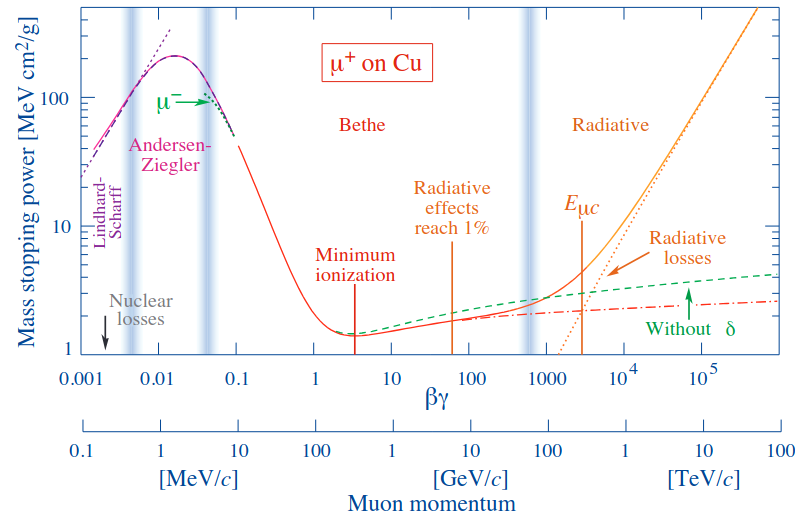
\includegraphics[width=0.7\linewidth]{Cuerpo/Ch_01/Interaccion_01.png}
\end{figure}
las partículas cargadas incrementan su pdoer de frenado drásticamente antes de frenarse en el medio, resultando en una gran deposición de energía antes de pararse, denominada \textbf{pico de Bragg}. Esto no ocurre en partículas ligeras (electrón) ni en el caso de radiación electromagnética. 


     
\subsection{Intreacciones de los fotones}



\subsection{Interacciones de los neutrones}

\section{Detectores}

En esta parte nos focalizaremos en la interacción de una partícula/radiación con el detector. Dicha interacción supone un efecto, en general la trasferencia de energía al medio. La forma en la que se trasfiere, y la conversión de esa trasnferencia en una señal útil es en lo que se diferencian los detectores. 

Los observables más interesantes son: contaje, tipo de partícula, energía depositada (espectroscopía), posición (tracking)... Y todos ellos en cierto modo dependen de la energía depositada en el medio, ya que es esta trasferencia de información la que puede decirnos que tipo de partícula es (por ejemplo, los electrones depositarán diferente energía que los protones en un medio), la posición de la interacción (ya que por ejemplo se generán fotones y se podrá obtener a través de extrapolación), contaje... 

En función de las formas de observación de la trasferencia de en la señal util tendremos observaciones ópticas u observaciones electrónicas. Los mecanismos de intreacción son: ionización, interacción con semiconductores, centelleo y reacción nuclear (captura, fisión, trasferencia...). Nosotros estudiaremos los detectores en función de la interacción, viendo en cada uno de estos que tipo de formas de observación hay. 

\subsection{Detectores de ionización}

Un detector de ionización es un gas formado por moléculas/átomos X tal que el paso de una partícula P (por ejemplo un núcleo, un electrón o un fotón) provoca que un del núcleo X se libere obteniendo un electrón libre y un ion cargado positivamente:

\[ \ce{P + X+ -> P +  X+ + e-} \]
También es posible que en la interacción P-X la molécula X se excite, y luego esta en la interacción con otra molécula la ionice, tal que: 

\[ \ce{P + X -> P +  X^* + e-} \quad \Longrightarrow \quad  \ce{X^* + Y -> X + Y^+ + e-}  \]
a lo primero lo llamamos \textbf{ionización primaria}, y a lo segundo \textbf{ionización secundario}. Este proceso podría repetirse para una ionización terciaria, cuaternaria... En la siguiente imagen tratamos de ilustrar mejor el concepto: 

\begin{minipage}{0.45\linewidth} \centering
    \captionof{figure}{Radiacion ionizante primaria \cite{DetectoresTECIV}.}
    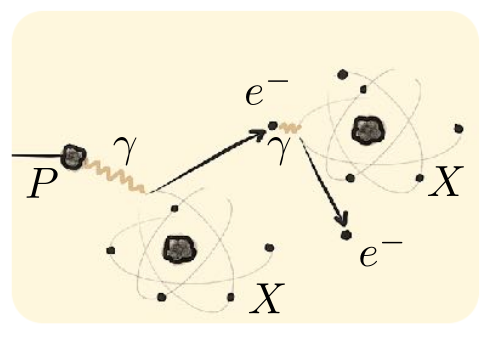
\includegraphics[width=0.9\linewidth]{Cuerpo/Ch_01/Detectores_01.png}
\end{minipage}
\hfill
\begin{minipage}{0.45\linewidth} \centering
    \captionof{figure}{Radiacion ionizante secundaria \cite{DetectoresTECIV}.}
    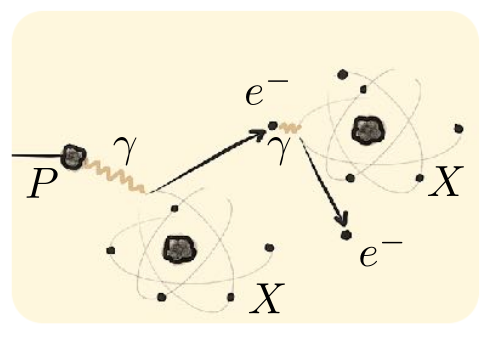
\includegraphics[width=0.9\linewidth]{Cuerpo/Ch_01/Detectores_01.png}
\end{minipage}




El valor de interés aquí será el número de pares creados, peus depende de  la energía depositada. Una vez se produce estos pares, y se ioniza el medio, es posible que aparecan \textit{nuevos mecanismos de ionización}: 

\begin{itemize}
    \item La \textit{trasferencia de carga} tal que:

    \[ \ce{ Y + X^+- -> X + Y^+-} \]

    \item El \textit{attachment}, en el que:
    \[ \ce{X + e- -> X^- + h \nu} \]

    \item La \textit{recombinación}: 
    \[ \ce{X^+ + e- -> X + h \nu} \]
\end{itemize}

En función del tipo de gas X que tengamos un mecanismo prevalecerá más que otro. tenemos básicamente 3 tipos de gases:

\begin{itemize}
    \item   Los \textbf{gases electronegativos}, que atrapan electrones (es decir, favorecen el proceso attachment). No se usan solos en detectores donde necesitas recoger electrones (ej. TPCs), pero sí pueden usarse para controlar descargas. Ejemplos: O$_2$,  H$_2$O, CO$_2$, CCl$_4$, SF$_6$.
    \item Los \textbf{gases ``quencher''} que atrapan o intreaccionan con fotones, en general  absorben fotones UV emitidos en procesos de excitación o recombinación. Evitan que esos fotones vuelvan a ionizar el gas, i.e. controlan descargas secundarias. Son en general gases orgánicos CH$_4$, C$_4$H$_{10}$, CO$_2$, CCl$_4$, SF$_6$. 
    \item Los \textbf{gases electropositivos} (``suelta electrones''). Son fáciles de ionizar, liberan electrones con poca energía, muy usados como gases base en detectores. No hacen attachment, por lo que presentan buena recolección de carga y resolución. Son en general \textit{gases nobles}: He, Ne, Ar, Xe, etc.
\end{itemize}   

Para el correcto funcionamiento de los detectores de ionización es necesario un proceso que aumente el número de iones y que se muevan para ser recogidos por otro detector que transifera la información. Para esto tenemos dos procesos: la creación de avalanchas y multiplicación:

\begin{itemize}
    \item En las \textbf{avalanchas} la energía de los electrones primarios es suficiente para ionizar el gas exponencialmente. Se pierde información acerca del número de electrones primarios.
    \item Cuando el fenómeno es la \textbf{multiplicación}, el campo aumenta gradualmente acelerando los electrones y creando multiplicación de las cargas. El número de electrones primarios es proporcional a los recogidos. 
\end{itemize}

Existen varios tipos de detectores por ionización: 

\begin{itemize}
    \item La \textbf{camara de ionización} contiene gases nobles, que producen una señal con carga proporicional a la energía perdida en el gas. 
    \item El \textbf{concator proporcional} es un mezclado de gases ``quencher'' y/o electronegativos. La forma del campo eléctrico acelera los elecctrones y produce ionización secundaria, siendo la señal proporcional al número de electrones (de ahí el nombre). 
    \item El \textbf{Geiger-Müler} es un mezclado de gases ``quencher'' y nobles, de tal modo que los gases ``quencher'' extinguen ionizaciones pequeñas. El campo electrico altísimo produce avalanchas en cadena, con señales independientes de la energía depositida y del tipo de partícula (se pierde esta información, solo existe detección, con muy alta eficiencia). Esta eficiencia depende de la partícula: para iones es del 100\%, para electrones muy alta y para fotones baja, $<10\%$. 
\end{itemize}
Como podemos ver, los diferentes detectores se ubican en regiones  diferentes de la siguiente imagen: 

\begin{figure}[H] \centering
    \captionof{figure}{Producción de pares de iones en función del voltaje aplicado.}
    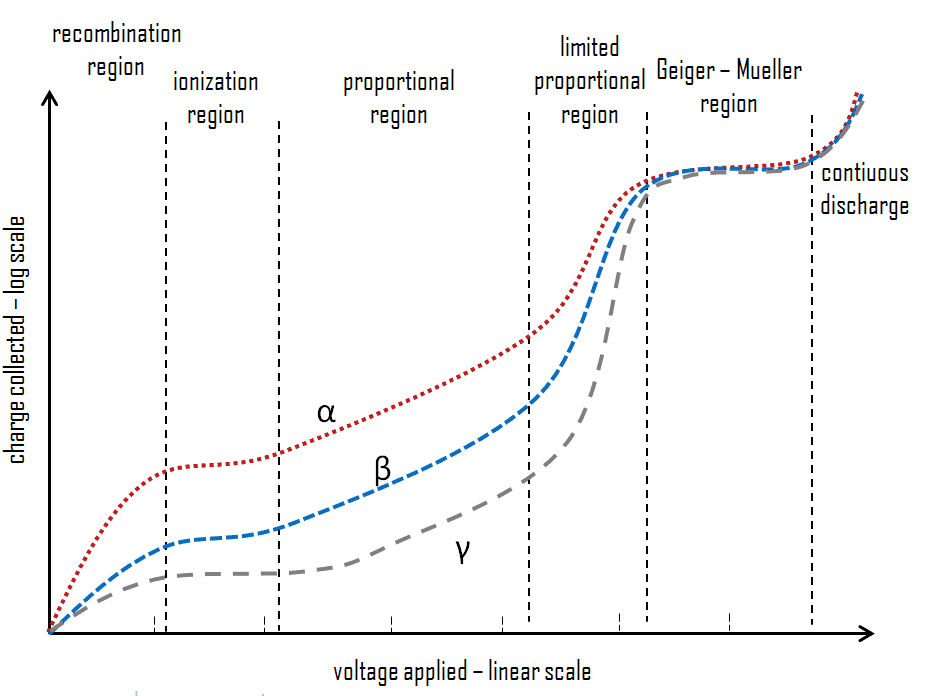
\includegraphics[width=0.7\linewidth]{Cuerpo/Ch_01/Detectores_03.png}
\end{figure}


\subsection{Detectores electrónicos: semiconductores}

Los detectores electrónicos basados en semiconductores, aprovechan la estructura de bandas y de valencia (Si, Ge) logicamente dopados, formando uniones PN. El principio es sencillo: cuando una partícula ioniza el material, crea pares de electrón-hueco, que son llevados en direcciones opuestas y recolectadas en los bordes del detector. 

La creación de huecos-electrones será más eficiente si ocurre en la zona de vaciamiento de una unión PN, ya que en esta región el alto campo eléctrico que hay (siempre y cuando apliquemos voltaje inverso en los extremo) hará que rapidamente se muevan y no se puedan recombinar. Uno puede deducir que la polarización en la que queremos la unión será inversa: región de vaciamiento más ancha y campo más alto. La señal se forma con la recollección de la carga, por lo que aparecerán dos componentes, una para los huecos y otra para los electrones. 


\subsection{Detectores de Centelleo}

El principio es sencillo: convierte la energía cinética de las partículas en luz (fotones), cuya intensidad es proporcional a la energía depositada.  Esto se produce porque el material absorbe parte de la energía de la partícula incidente (quedando ``excitado'' durante un tiempo determinado) y la reemite en forma de un corto destello de luz, típicamente en el rango de la luz visible. El medio será trasparente a la longitud de onda de su propia emisión, ya que en caso contrario se producirá dispersión de la luz. 


En función del tiempo de excitación del material:

\begin{itemize}
    \item La \textbf{fluorescencia} tiene tiempos de exctiación (medios) tal que $\tau_{1/2} <$ ps, siendo transiciones atómicas.
    \item La \textbf{fosforescencia} tiene tiempos de exctiación (medios) tal que $\tau_{1/2}$ de $\mu$s a h.
\end{itemize}
Pueden ser ópticos (espintariscopio, Geiger Marsden) o eléctricos, en los que se usan dispositivos multiplicadores para aumentar la señal. Esto último es lo más usado, ya que proporcionan una mayor sensibilidad a la energía, respuesta rápida (ns) y la posibilidad de análisis de pulsos. Distinguimos dos clases de materiales de los que puede estar hecho el centelleador:

\begin{itemize}
    \item Los materiales \textbf{inorgánicos}, como estructuas cristalinas (NaI(Tl), CsI(Tl,Na)...), cristales amorfos o gases nobles. Estos presentan mejor respuesta lumínica (correspondencia lineal con la energía) pero son más lentos.
    \item Los materiales \textbf{orgánicos} que pueden ser líquidos o sólidos (cristales o plásticos). Son más rápidos pero emiten menos cantidad de luz. 
\end{itemize}


Los tubos fotomultiplicadores, por otro lado, pueden ser de 3 tipos: 

\begin{itemize}
    \item \textbf{Fotocátodos:} sería un semiconductor junto con un metal alcalino, capaz de convertir la radiación dentro del rango últil del espectro en electrones.
    \item \textbf{Sistema de entrada electro-óptica}: recolección electrónica eficiente. Es independiente de la posición y posee buena resolución en tiempo. 
    \item \textbf{Sección de multiplicación electrónica}: compuesta por varios  dínodos\footnote{Un dínodo es el nombre que reciben cada uno de los electrodos de un tubo fotomultiplicador. Cada dínodo está cargado más positivamente unos 100 voltios que su predecesor, de tal forma que cuando el fotocátodo del tubo recibe un fotón y consecuentemente emite un electrón, este se dirige al primer dínodo, el cual recibe el impacto del electrón en su superficie, emitiendo en un proceso secundario, a su vez más electrones que se dirigen al siguiente dínodo. Y así sucesivamente hasta llegar al ánodo receptor. De esta forma, son capaces de aumentar hasta un millón de veces la pequeña corriente emitida por el fotocátodo, produciéndose de 105 a 107 electrones por cada fotón incidente. \cite{wiki-dinodo}.}, el potencial se incrementa con cada dinodo hasta el ánodo. La multiplicación en cada etapa resulta en una ganancia neta.    
    \item \textbf{Fotomultiplicadores de avalancha:} aprovechan las características de un semiconductor para crear un campo eléctrico de deriva y multiplicación.
\end{itemize}

\begin{figure}[H] \centering
    \caption{fotomultplicador de avalancha, donde se ven los dinodos (\textit{dynoden}).}
    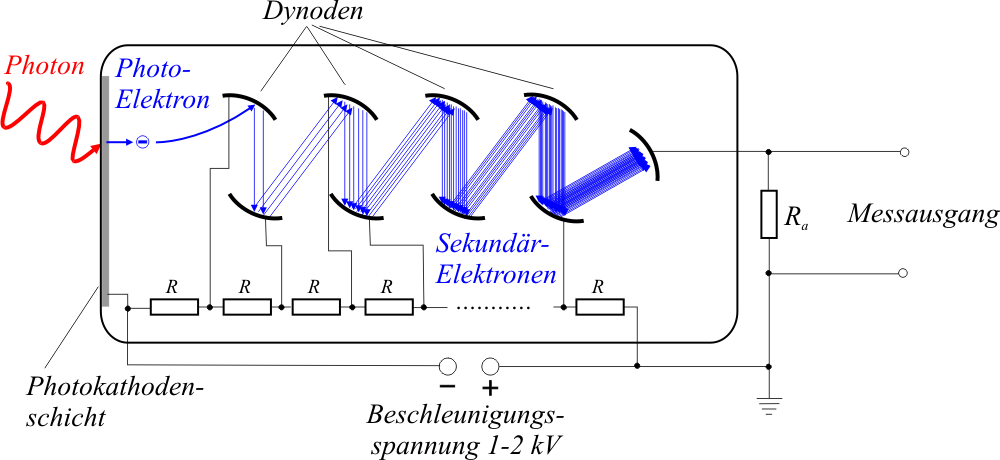
\includegraphics[width=0.7\linewidth]{Cuerpo/Ch_01/Detectores_Fotomultiplicador.png}
\end{figure}

\subsection{Montaje electrónico}

En el montaje, una vez ocurre la detección y se produce la señal, esta debe ser amplificada, tratada, y/o discriminada. Luego, debe codificarse para que sea digital y se muestre de la manera adecuada . Las partes son: 

\begin{enumerate}
    \item \textbf{Preamplificación:} sensible a la carga, voltaje o intensidad (básicamente la señal que llega), filtrando la parte del ruido y frecuencias no deseadas. 
    \item \textbf{Amplificación:} segunda amplificación, tratando la señal y modifica su forma en función de sus características.
    \item \textbf{Discriminador:} envía una señal lógica cuando la señal de entrada supera un cierto umbral.
    \item \textbf{Codificación en canales} cada medida es una cuenta que se puede acumular en un histograma. 
\end{enumerate}


\subsection{Características de los detectores}

Las condicinoes de funcionamiento dependen de las características del detector: tipo de detector, material, presión, temperautra... Así pues, tenemos varias características que nos pueden ayudar a discernir (buena resolución, calibración amplia y duradera, buena eficiencia...) un buen detector de un mal detector:

\begin{itemize}
    \item \textbf{Calibración:} puede ser en energia, tiempo o posición. En el caso de la energía se traducen los canales a unidades de energía, haciendo una correspondencia lineal con una fuente que emita a energías bien definidas.
    \item \textbf{Resolución:} en general se refiere a la relación entre el ruido del detector y la electróncia asociada con el valor dado. En particular podemos distinguir: en energía ($\Delta E / E$), asociada a fluctuaciones estadísticas en la fomración de portadores de carga/deposición de energía o la colección incompleta de la carga producida; en tiempo ($\Delta t / t$), asociada a la formación del pulso y el proceso de discriminación; o a la posición ($\Delta x / x$) asociado al tamaño y geometría de las celdas.
    \item \textbf{Eficiencia total:} para tener buena eficiencia la partícula debe alcanzar el medio activo del detector, transferir la energía al medio activo o convertir  la inforamción en señal útil. La definimos como

    \begin{equation}
        \varepsilon_{tot} = \frac{\text{nº de sucesos detectados}}{\text{nº de sucesos emitidos}}
    \end{equation}
    Depende de la geometría, probabilidad de interacción y tipo de radiacción. Asi pues distinguimos:

    \begin{equation}
        \varepsilon_{tot} = \varepsilon_{intr} \cdot \varepsilon_{geo}
    \end{equation}
    definiendo: 

    \begin{equation}
        \varepsilon_{geo} = \frac{\text{nº de sucesos que llegan al detector}}{\text{nº de sucesos emitidos}}
    \end{equation}
    \begin{equation}
        \varepsilon_{intr} = \frac{\text{nº de sucesos detectados}}{\text{nº de sucesos que llegan al detector}}
    \end{equation}
    \item \textbf{Tiempo muerto:} es el tiempo mínimo entre dos señales discernibles, dependiento de la respuesta del dector y la cadena electrónica. Es fundamental estudiar que significa que neustro detector sea paralizable o no paralizable.  Sea $\tau$ el tiempo muerto, $n$ la tasa real y $m$ la tasa detectada.
    
    \begin{itemize}
        \item \textbf{Detector paralizable}: como indica su palabra, reinicia la deetección cada vez que hay una nueva detección. sea $t_0$ el instante de la detección y sea $t_1$ es la de la segunda detección. Si $t_1<t_0+\tau$, entonces el detector paralizable reiniciará la cuenta y solo realizará una detección, siempre y cuando otra detección $t_3$ verifique que $t_3<t_2+\tau$, porque en ese caso volverá a reiniciarse. En este caso:
        \begin{equation}
            m = \frac{m}{1+m\tau}
        \end{equation}
        \item \textbf{Detector no paralizable}: como indica su palabra, no reinicia la deetección cada vez que hay una nueva detección. Sea $t_0$ el instante de la detección y sea $t_1$ es la de la segunda detección. Si $t_1<t_0+\tau$, entonces el detector no paralizable no detectará la cuenta, y solo realizará una detección, sin embargo en este caso si hay una tercera detección será detectado siempre que $t_3<t_1+\tau$. 
        \begin{equation}
            m = n e^{-n \tau}
        \end{equation}
    \end{itemize}
    Como podemos ver la tasa detecada del no paralizable es mayor que la del paralizable: 
    \begin{figure}[H] \centering
        \caption{tasa de detecciones vs eventso reales para detectores no paralizables y paralizables \cite{Knoll:1300754}.}
        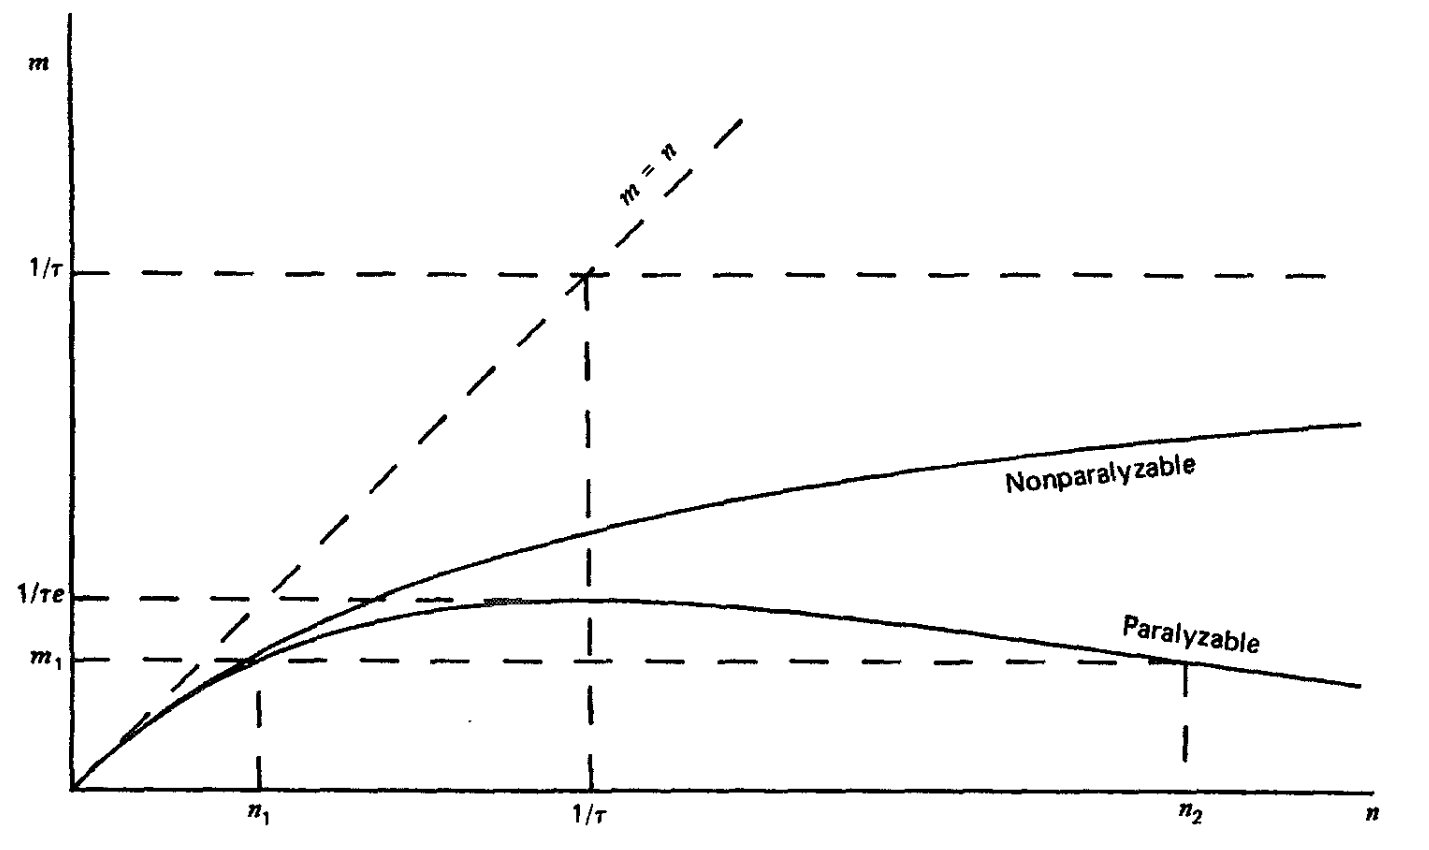
\includegraphics[width=0.7\linewidth]{Cuerpo/Ch_01/Detectores_muerto.png}
    \end{figure}
    
\end{itemize}
